\section{Auswertung}
\label{sec:Auswertung}

\subsection{Vorbereitung}

Die Größen Ordnungszahl $Z$, Literaturwert der
K-Kante $E_\text{K}^\text{Lit}$, der zugehörige Glanzwinkel 
$\theta_\text{glanz}^\text{Lit}$ und die Abschirmkonstante 
$\sigma_\text{K}$ verschiedener Elemente in Tabelle 
\ref{tab:literatur} aufgelistet.

\begin{table}
  \centering
  \caption{Literaturwerte und daraus errechnete Größen verschiedener Elemente}
  \label{tab:literatur}
  \sisetup{table-format=2.1}
  \begin{tabular}{c c c c c}
  \toprule
  $ $ & $Z$ & $E_\text{K}^\text{Lit} \,/\, \si{\kilo\eV}$
  & $\theta_\text{glanz}^\text{Lit} \,/\, \si{\degree}$ & 
  $\sigma_\text{k}$\\
  \midrule 
  Zn & 30 & 09,65 & 18,60 & 3,56 \\
  Ge & 32 & 11,10 & 16,10 &  \\
  Br & 35 & 13,47 & 13,22 &  \\
  Rb & 37 & 15,19 & 11,69 &  \\
  Sr & 38 & 16,10 & 11,03 &  \\
  Zr & 40 & 18,00 & 09,85 &  \\
  Nb & 41 & 18,99 & 09,33 &  \\
  Au & 49 &  &  &  \\
  \bottomrule
  \end{tabular}
  \end{table}




\subsection{Überprüfung der Bragg Bedingung}

Nach der Braggbedingung ist zu erwarten, dass das gemessene Intensitätsmaximum
für den errechneten Glanzwinkel auftritt. 

Die Berechnung erfolgt über die Umstellung der Gleichung \eqref{eqn:Bragg} zum Glanzwinkel
hin und durch Einsetzen des Ausdrucks $\lambda = \frac{h \cdot c}{E}$ zu 

\begin{equation}
  \theta_\text{glanz} = \text{arcsin}\left(\frac{h \cdot c}{E \cdot 2d}\right)
  \label{eqn:theta}
\end{equation}

Mit einer Gitterkonstanten $d_\text{LiF} = \SI{201.4}{\pico\meter}$ und den Energien

\begin{align*}
   \text{Für } K_\alpha \text{ : } E_{K_\alpha} &= \SI{8.046}{\kilo\eV} \\
   \text{Für } K_\beta \text{ : } E_{K_\beta} &= \SI{8.904}{\kilo\eV}
\end{align*}

ergeben sich aus der Gleichung \eqref{eqn:theta} die Glanzwinkel

\begin{align*}
  \theta_{K_\alpha} &= \SI{22.49}{\degree} \\
  \theta_{K_\beta} &= \SI{20.22}{\degree} \: .
\end{align*}

Aus Abbildung ... erhält man für die Stellen der beiden Peaks etwa $\SI{40}{\degree}$
und $\SI{45}{\degree}$. Beachtet man die Skalierung des Winkels, so ist
erkennbar, dass die experimentell bestimmten Glanzwinkel minimal von den Sollwinkeln
abweichen. Die Braggbedingung trifft folglich zu.

\subsection{Das Emissionsspektrum einer Kupferröntgenröhre}








%\begin{figure}
%  \centering
%  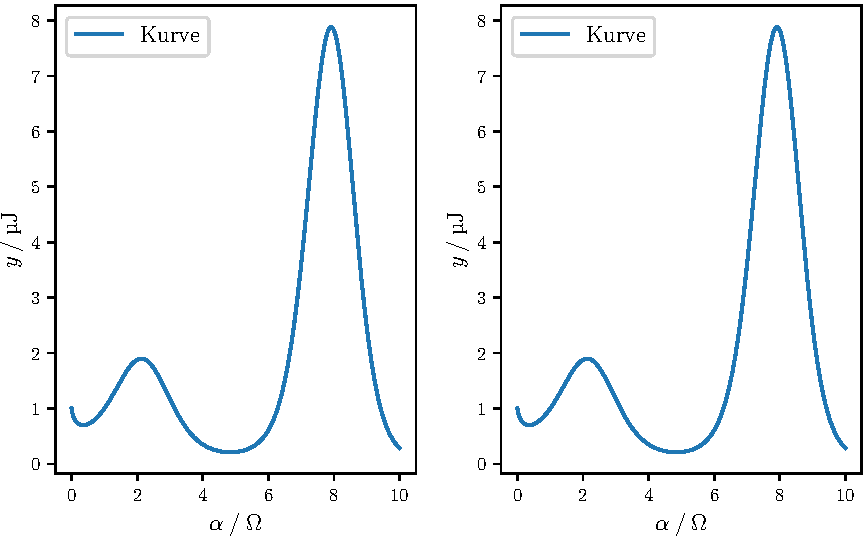
\includegraphics{plot.pdf}
%  \caption{Plot.}
%  \label{fig:plot}
%\end{figure}
